\newpage
\section{Simulation Environment}
\label{sec:simulation}

\subsection{Open-Source Foundation}
\label{subsec:simulation-overview}

The simulator used in this study is a research extension of the open-source PureEdgeSim line, introduced by Mechalikh et al. as a modular discrete-event framework for cloud, edge, and mist computing evaluation \cite{mechalikh2021pureedgesim, pureedgesimgithub}. For the present work, this foundation is particularly suitable because it already models heterogeneous devices, mobility, task generation, networking, and orchestration within a unified experimental environment.

The 2021 PureEdgeSim paper further describes a layered architecture built on top of CloudSim Plus, with dedicated managers for simulation control, data-center generation, task generation, mobility, networking, and orchestration \cite{mechalikh2021pureedgesim, silvafilho2017cloudsimplus}. This modular decomposition is central to the current project. It provides the event-driven backbone, configuration pipeline, logging support, and heterogeneous infrastructure model needed for edge-cloud experiments, allowing the implementation effort to focus on scheduling and network extensions rather than on rebuilding a simulator from first principles.

The later comparative study by Mechalikh et al. evaluates 24 edge simulators and reports that PureEdgeSim remains among the actively maintained tools while also exhibiting strong scalability and reliability characteristics \cite{mechalikh2025quality}. For a report centered on scheduling methodology, such a stable open-source base is preferable to a bespoke simulator with no external pedigree. The implementation used here follows the CloudSim-Plus-based PureEdgeSim line, with PureEdgeSim 4.2.0 and CloudSim Plus 6.2.7 as the immediate software foundation.

\subsection{Relation to Prior PureEdgeSim-Based RL Systems}
\label{subsec:customized-environment}

The studies by Robles-Enciso and Skarmeta are the most relevant precedents because they show that PureEdgeSim can be extended beyond heuristic orchestration and used as a reinforcement-learning testbed \cite{robles2022continuum, robles2023multilayer}. In their 2022 conference paper and 2023 journal version, PureEdgeSim v4.2 is adapted to evaluate greedy, single-layer RL, and multi-layer guided RL policies for task offloading in a computing continuum. Their experiments use a \(200\,\mathrm{m} \times 200\,\mathrm{m}\) scenario, an edge--fog--cloud hierarchy, repeated random simulations, and metrics such as task success rate, average total time, latency failures, CPU usage, and energy consumption. These studies establish that PureEdgeSim can support repeated RL evaluation over heterogeneous multi-tier infrastructures.

The environment required here, however, differs in both architecture and decision space. Robles-Enciso and Skarmeta focus on task assignment across local, edge, fog, and cloud processing nodes, and their agents choose offloading destinations without an explicit radio-resource action space \cite{robles2022continuum, robles2023multilayer}. The present work instead targets a LOCAL--EDGE--CLOUD architecture and treats wireless Physical Resource Block (PRB) reservation as part of each decision. The simulator is therefore extended not merely to host RL logic, but to support joint communication-and-computation control under deep on-policy learning.

The resulting project-specific extensions and their placement in the software stack are summarized in \Figref{fig:pureedgesim-extensions}. Rather than adding isolated utilities, the project extends PureEdgeSim through four coordinated layers around the original simulator stack.
\begin{enumerate}[(a)]
    \item \textbf{Simulator-side environment extensions.} On the Java side, the customized environment integrates PRB-aware wireless resource management, device-level observation and reward construction, and a unified orchestration path so that joint communication-and-computation decisions remain embedded in the original event-driven simulator loop.
    \item \textbf{RL interface layer.} The simulator exposes decision points to Python through an orchestration hook, a device-level decision-support module, and \texttt{RLEnvServer}, which together provide a synchronous JSON-over-TCP interface for MAPPO and PPO policies.
    \item \textbf{Runtime execution support.} \texttt{AbstractRLManager} unifies external training mode and offline inference mode, including Python process launch, connection management, model-path handling, and failure fallback.
    \item \textbf{Telemetry and evaluation support.} The environment exports trajectory CSV files, seed-wise summaries, and RL-specific charts for destination usage, PRB usage, and reward evolution, thereby supporting training diagnostics, reproducibility, and post-run policy analysis.
\end{enumerate}

\begin{figure}[htbp]
    \centering
    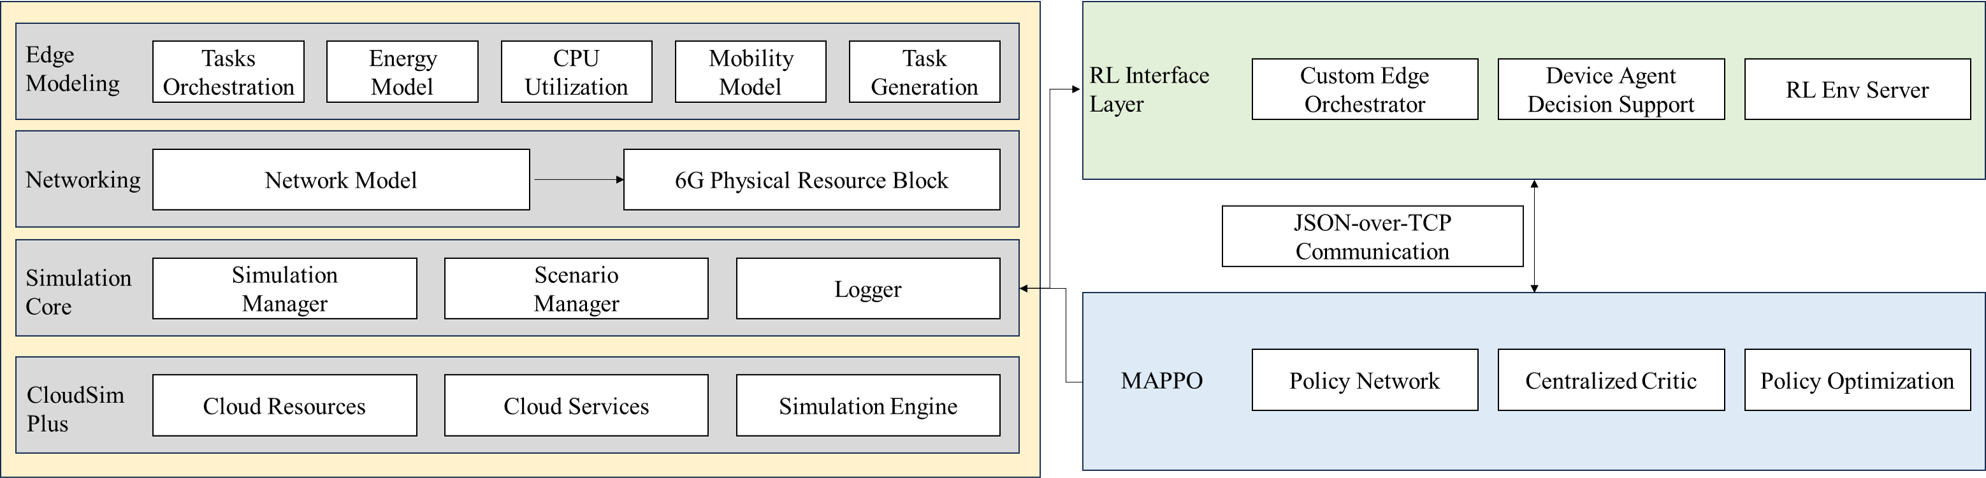
\includegraphics[width=\textwidth]{figures/extended_pureedgesim_rl_architecture.png}
    \caption{Extended PureEdgeSim software stack with the RL interface layer and the MAPPO decision components used in the project environment.}
    \label{fig:pureedgesim-extensions}
\end{figure}

\subsection{Instantiated Experimental Environment}
\label{subsec:simulation-configuration}

This subsection records the concrete simulator instance used in the experiments. The formal communication, computation, energy, and reward models are deferred to \Secref{sec:system-model}; the emphasis here is on how the environment is instantiated for empirical evaluation.

The scenario comprises 160 devices in a \(200\,\mathrm{m} \times 200\,\mathrm{m}\) area, four edge data centers, and one cloud node. The simulation horizon is 30 minutes, deliberately longer than in the Robles studies so that each episode produces tens of thousands of scheduling decisions and exposes the policies to sustained congestion and mobility effects. The resulting setup remains close enough to prior PureEdgeSim practice for comparison, while being specialized to the LOCAL--EDGE--CLOUD architecture studied here.

\begin{table}[htbp]
    \centering
    \begin{tabular}{p{0.48\linewidth}p{0.32\linewidth}}
        \hline
        \textbf{Parameter} & \textbf{Value} \\
        \hline
        Simulation area & \(200\,\mathrm{m} \times 200\,\mathrm{m}\) \\
        Number of devices & 160 \\
        Simulation time & 30 min \\
        Mobile device speed & \(1.4\,\mathrm{m/s}\) \\
        Edge-device communication range & \(40\,\mathrm{m}\) \\
        Edge data-center coverage radius & \(120\,\mathrm{m}\) \\
        Cloud equivalent distance & \(160\,\mathrm{m}\) \\
        WLAN bandwidth & \(5000\,\mathrm{Mbps}\) \\
        Total PRB blocks & 5000 \\
        Reference distance \(d_0\) & \(20\,\mathrm{m}\) \\
        Distance exponent \(\alpha\) & 0.5 \\
        Maximum PRBs per task & 50 blocks \\
        VM scheduling policy & \texttt{SPACE\_SHARED} \\
        Random-seed set for final evaluation & 9001, 9002, 9003 \\
        \hline
    \end{tabular}
    \caption{Main simulator parameters used in the reported experiments.}
    \label{tab:simulation-parameters}
\end{table}

Only devices with \texttt{generateTasks=true} are treated as RL agents. In the instantiated workload, these are the smartphones and sensors. This choice follows the PureEdgeSim practice used in the Robles studies, where learning is attached to actual task initiators rather than to every simulator entity. Non-agent devices still affect the environment through mobility, compute competition, and shared wireless contention, so the overall system remains strongly coupled.

\subsection{Event-Driven Task Lifecycle}
\label{subsec:task-orchestration-flow}

PureEdgeSim remains event-driven rather than being recast as a fixed-step game loop \cite{mechalikh2021pureedgesim}. The present project preserves that design. Decisions are triggered only when tasks arrive at the orchestration stage, not at an artificial global clock tick, so the simulator retains its original temporal semantics.

Once a task is generated, it is sent to the orchestrator, which selects the execution destination and, for RL-based algorithms, the PRB level used for the wireless upload. The task is then transmitted to the chosen destination, executed on the assigned VM, and finally returned to the source device. \Figref{fig:task-orchestration-flow} summarizes this simulator-side lifecycle.

\begin{figure}[htbp]
    \centering
    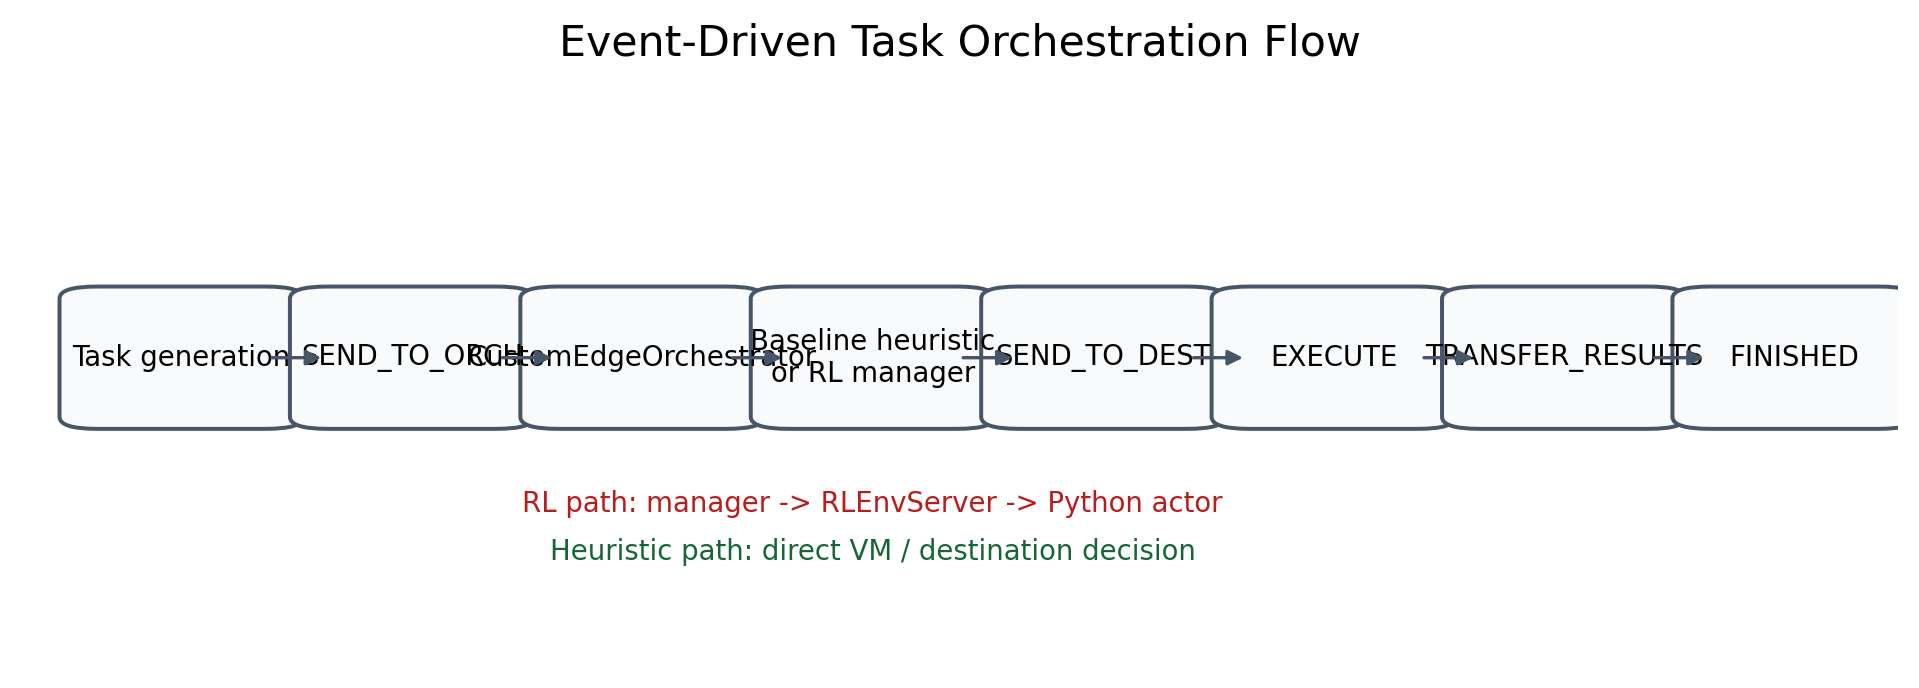
\includegraphics[width=0.92\textwidth]{figures/task_orchestration_flow.png}
    \caption{Simulator-side event-driven task lifecycle in the customized environment.}
    \label{fig:task-orchestration-flow}
\end{figure}

For heuristic baselines, \texttt{CustomEdgeOrchestrator} computes the destination directly. For RL algorithms, the same orchestrator delegates the decision to \texttt{MAPPOManager} or \texttt{PPOManager}, which assemble the observation, query the Python policy, sanitize the returned action, and inject the selected destination and PRB allocation back into the event pipeline. All methods therefore operate inside the same PureEdgeSim lifecycle and are evaluated under the same task generator, mobility model, network model, and data-center configuration.

\subsection{Java-Python Co-Simulation Architecture}
\label{subsec:java-python-cosim}

\subsubsection{Training Mode}

Earlier PureEdgeSim RL studies place the learning logic inside the simulator loop \cite{robles2022continuum, robles2023multilayer}. The present project separates the discrete-event simulator and the learning components across Java and Python. In training mode, Python launches the Java simulator with the environment-server flag enabled. Java instantiates \texttt{RLEnvServer} and waits for the Python client to connect. The first message, \texttt{marl\_config}, communicates the number of agents, observation dimensions, destination labels, and PRB bins. Each decision then follows a request-response sequence:
\begin{align*}
\texttt{marl\_turn\_obs} \rightarrow \texttt{marl\_action} \rightarrow \texttt{marl\_transition},
\end{align*}
followed by \texttt{marl\_episode\_end} at the end of each episode.

This separation assigns complementary responsibilities to the two runtimes. Python handles inference, trajectory buffering, and policy updates, whereas Java remains authoritative for event timing, validity checks, fallback handling, and reward calculation. \Figref{fig:java-python-training-architecture} illustrates this training-time collaboration between simulator-side control flow and learner-side optimization.

\begin{figure}[htbp]
    \centering
    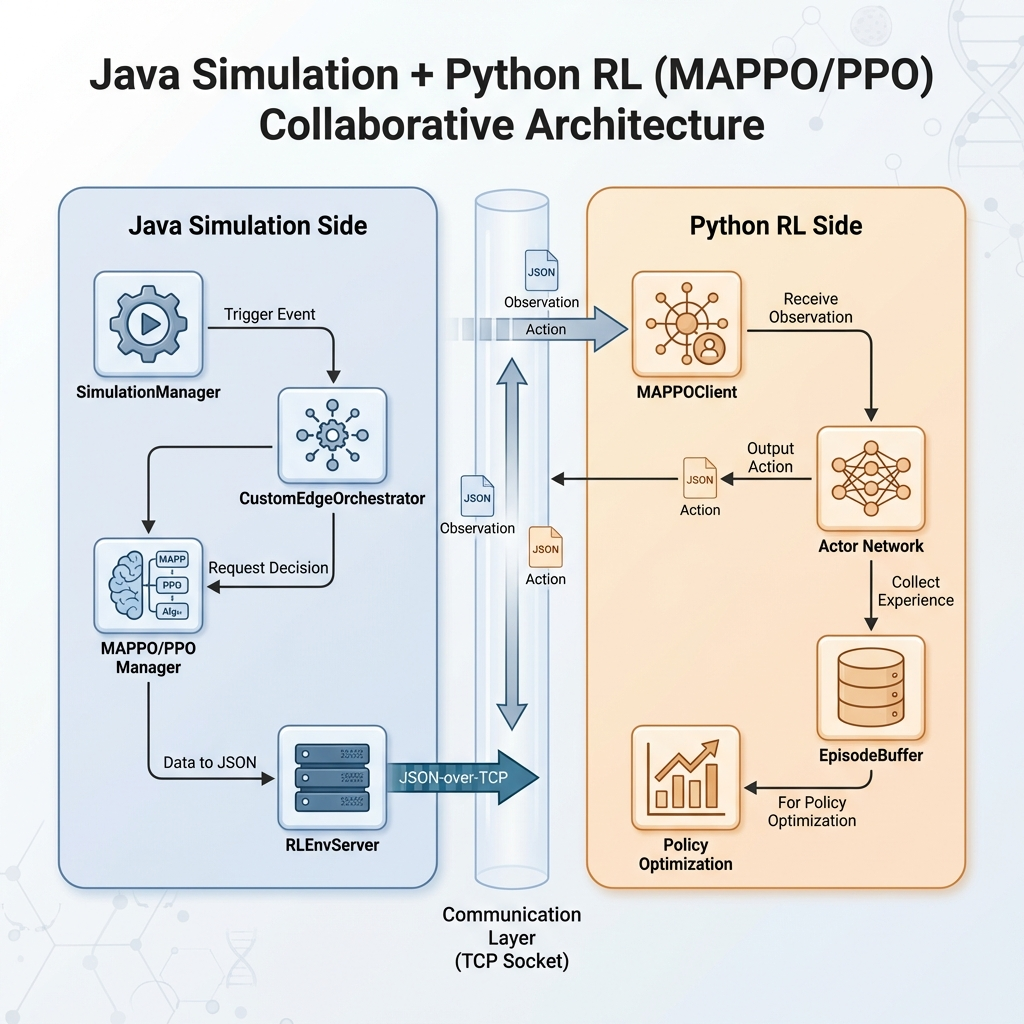
\includegraphics[width=0.92\textwidth]{figures/java_python_training_architecture.png}
    \caption{Training-time interaction between the Java simulator and the Python MAPPO/PPO learner.}
    \label{fig:java-python-training-architecture}
\end{figure}

\subsubsection{Offline Inference Mode}

In offline inference mode, Java automatically launches \texttt{inference\_server.py} and connects to it through the same TCP interface. The model path is resolved by priority: an explicitly supplied checkpoint is used first, otherwise the latest training run is searched, and finally a legacy fallback path is checked. If no checkpoint can be loaded, the manager falls back to a safe default action so that evaluation runs remain executable. \Figref{fig:java-python-cosim} summarizes the shared protocol and data flow reused by both training and offline inference.

\begin{figure}[htbp]
    \centering
    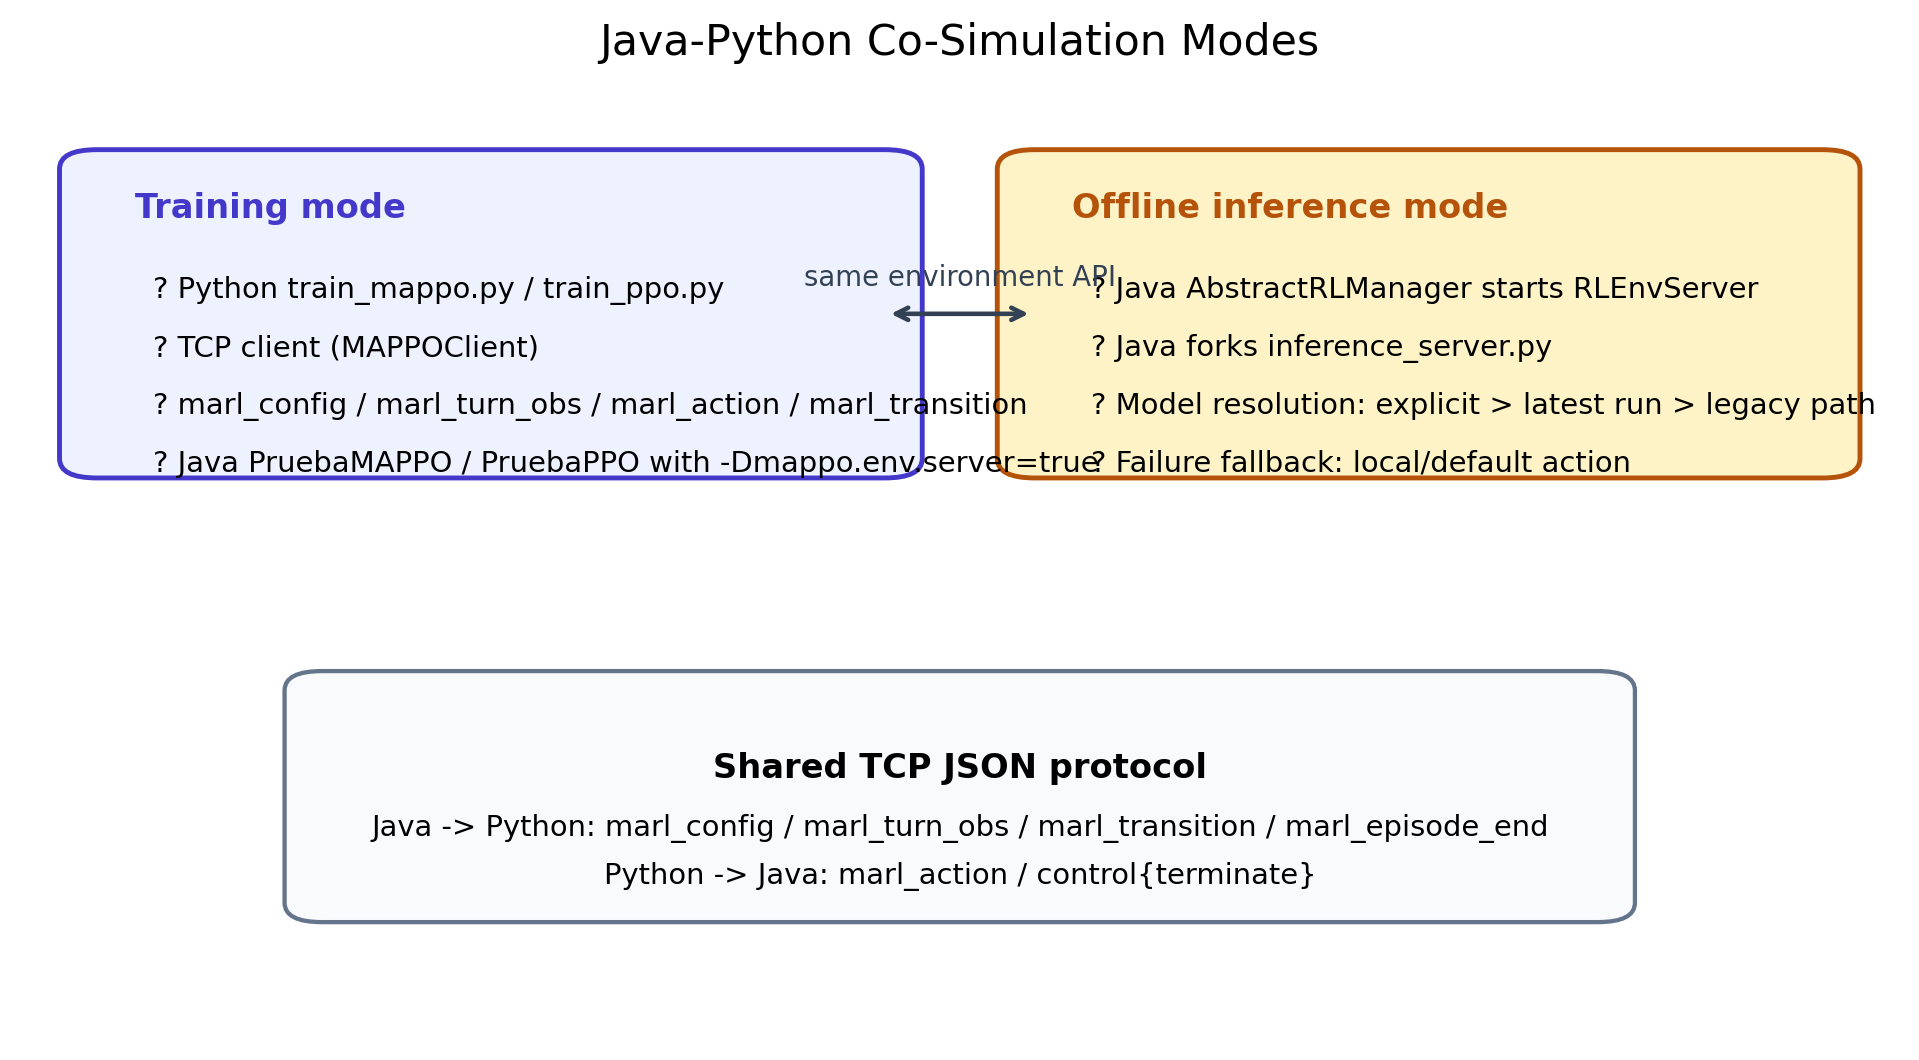
\includegraphics[width=0.92\textwidth]{figures/java_python_cosim.png}
    \caption{Shared Java--Python co-simulation interface used by training and offline inference.}
    \label{fig:java-python-cosim}
\end{figure}

The same message protocol is reused in both modes, so training and evaluation share a common environment interface. Reusing one interface reduces train-test skew and makes the RL pipeline easier to debug.

\subsection{Evaluated Scheduling Algorithms}
\label{subsec:baseline-algorithms}

The simulator is used to evaluate the proposed MAPPO policy against both heuristic and learning-based references. This follows the general evaluation logic of the Robles studies, where RL methods are judged against simpler alternatives rather than in isolation \cite{robles2022continuum, robles2023multilayer}. In total, MAPPO is compared against ten heuristic schedulers and one single-policy PPO variant. The heuristic set spans naive, locality-driven, load-driven, and multi-factor rules, while PPO serves as a learning baseline under the same environment and dual-action formulation.

\begin{table}[htbp]
    \centering
    \begin{tabular}{p{0.22\linewidth}p{0.68\linewidth}}
        \hline
        \textbf{Algorithm} & \textbf{Decision rule} \\
        \hline
        RANDOM & Randomly select a feasible VM. \\
        LOCAL & Prefer local execution and fall back to edge or cloud through a simple backup rule. \\
        CLOSEST & Choose the nearest edge node, with queue length as the tie-breaker. \\
        EDGE & Restrict execution to the edge tier and choose the least-loaded feasible VM. \\
        CLOUD & Restrict execution to the cloud tier and choose the least-loaded feasible VM. \\
        ROUND\_ROBIN & Select the VM with the smallest task count across all tiers. \\
        TRADE\_OFF & Use a weighted cost proportional to \((tasks+1)\times weight \times taskLength / vmMips\). \\
        INCREASE\_LIFETIME & Favor decisions that preserve device battery lifetime. \\
        LATENCY\_ENERGY\_AWARE & Combine delay and energy terms in a hand-crafted weighted policy. \\
        WEIGHT\_GREEDY & Minimize a normalized weighted sum of distance delay, execution delay, load, and energy. \\
        PPO & Single-policy PPO baseline that removes agent embeddings and shares one actor across all devices. \\
        \hline
    \end{tabular}
    \caption{Scheduling baselines evaluated in the customized orchestrator.}
    \label{tab:baseline-algorithms}
\end{table}

This distinction is important. PPO and MAPPO share the same PureEdgeSim-based environment and the same destination/PRB action structure, but MAPPO adds agent-specific embeddings and centralized multi-agent training over a global state. PPO therefore functions as a controlled baseline for isolating the contribution of the multi-agent design rather than as merely another RL competitor. Across all methods, the simulator side remains identical, preserving fairness of comparison.
